\section{采样接口}\label{sec:采样接口}
正如先在\refsub{应用到图像合成}介绍的,
pbrt中实现的渲染方法包含了在图像平面的2D点之外的额外维度上选择样本点。
各种算法将用于生成这些点,但它们的所有实现都继承自定义其接口的抽象类\refvar{Sampler}{}。
核心采样声明和函数在文件\href{https://github.com/mmp/pbrt-v3/blob/master/src/core/sampler.h}{\ttfamily core/sampler.h}
和\href{https://github.com/mmp/pbrt-v3/blob/master/src/core/sampler.cpp}{\ttfamily core/sampler.cpp}中。
样本生成的每种实现都在目录{\ttfamily samplers/}下其自己的源文件内。

\refvar{Sampler}{}的任务是生成$[0,1)^n$中$n$维样本的序列,
其中每个图像样本都要为其生成这样的样本向量,且每个样本中的维数$n$可能会变,
这取决于光传输算法执行的计算(见\reffig{7.13})。
\begin{figure}[htbp]
    \centering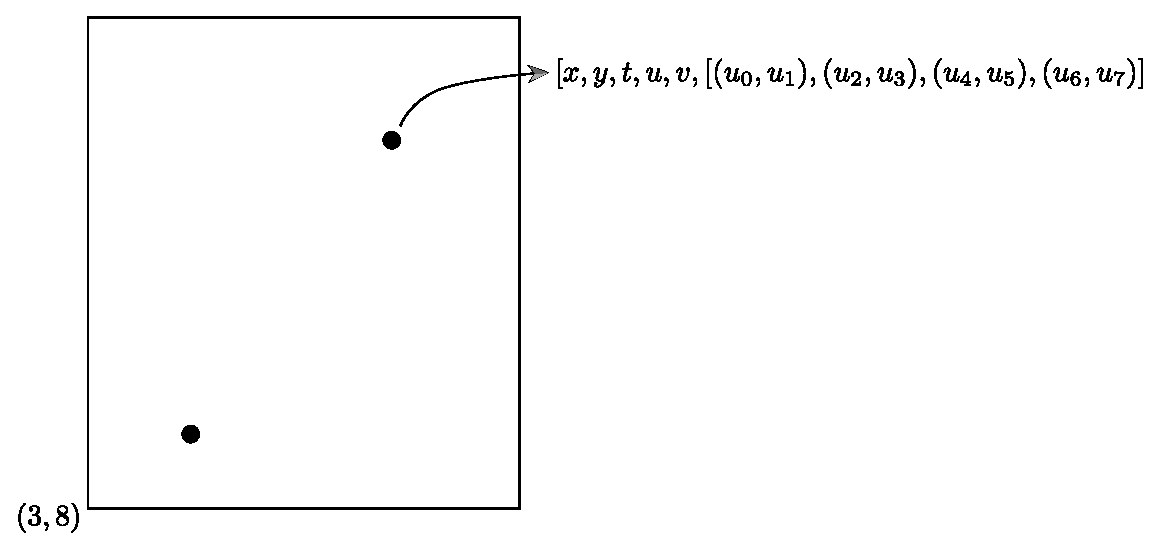
\includegraphics[width=0.9\linewidth]{chap07/Samplerndimensional.eps}
    \caption{采样器为每个图像样本生成用来合成最终图像的$n$维样本向量。
        这里,像素$(3,8)$正被采样,且在该像素区域内有两个图像样本。
        样本向量的前两维给出样本在该像素内的偏移量$(x,y)$,
        接下来三维决定相应相机光线的时间和透镜位置。后续维度用于
        第\refchap{光传输I:表面反射}、\refchap{光传输II:体积渲染}和\refchap{光传输III:双向方法}中
        的蒙特卡罗光传输算法。这里,光传输算法已经请求了样本向量中的四个2D数组样本;
        例如,这些值可能用于选择面光源上的四个点来为图像样本计算辐亮度。}
    \label{fig:7.13}
\end{figure}

因为样本值必须严格小于1,所以定义一个常数\refvar{OneMinusEpsilon}{}很有用,
它表示小于1的最大可表示浮点常数。然后,我们会截断样本向量值使之不大于该值。
\begin{lstlisting}
`\initcode{Random Number Declarations}{=}`
#ifdef PBRT_FLOAT_IS_DOUBLE
static const `\refvar{Float}{}` `\initvar{OneMinusEpsilon}{}` = 0x1.fffffffffffffp-1;
#else
static const `\refvar{Float}{}` OneMinusEpsilon = 0x1.fffffep-1;
#endif
\end{lstlisting}

可能最简单的\refvar{Sampler}{}实现是当每次需要样本向量的额外分量时直接返回$[0,1)$内的均匀随机值。
这样的采样器可产生正确的图像但会需要非常多的样本(以及更多要追踪的光线与更多的时间)来
创建用更先进采样器所能取得的相同质量的图像。
使用更佳采样模式的运行时间开销大致和用诸如均匀随机数的低质量模式相同;
因为为每个图像样本计算辐亮度比计算样本的分量值会有大得多的开销,
所以这样做是有回报的(\reffig{7.14})。
\begin{figure}[htbp]
    \centering
    \subfloat[差的采样]{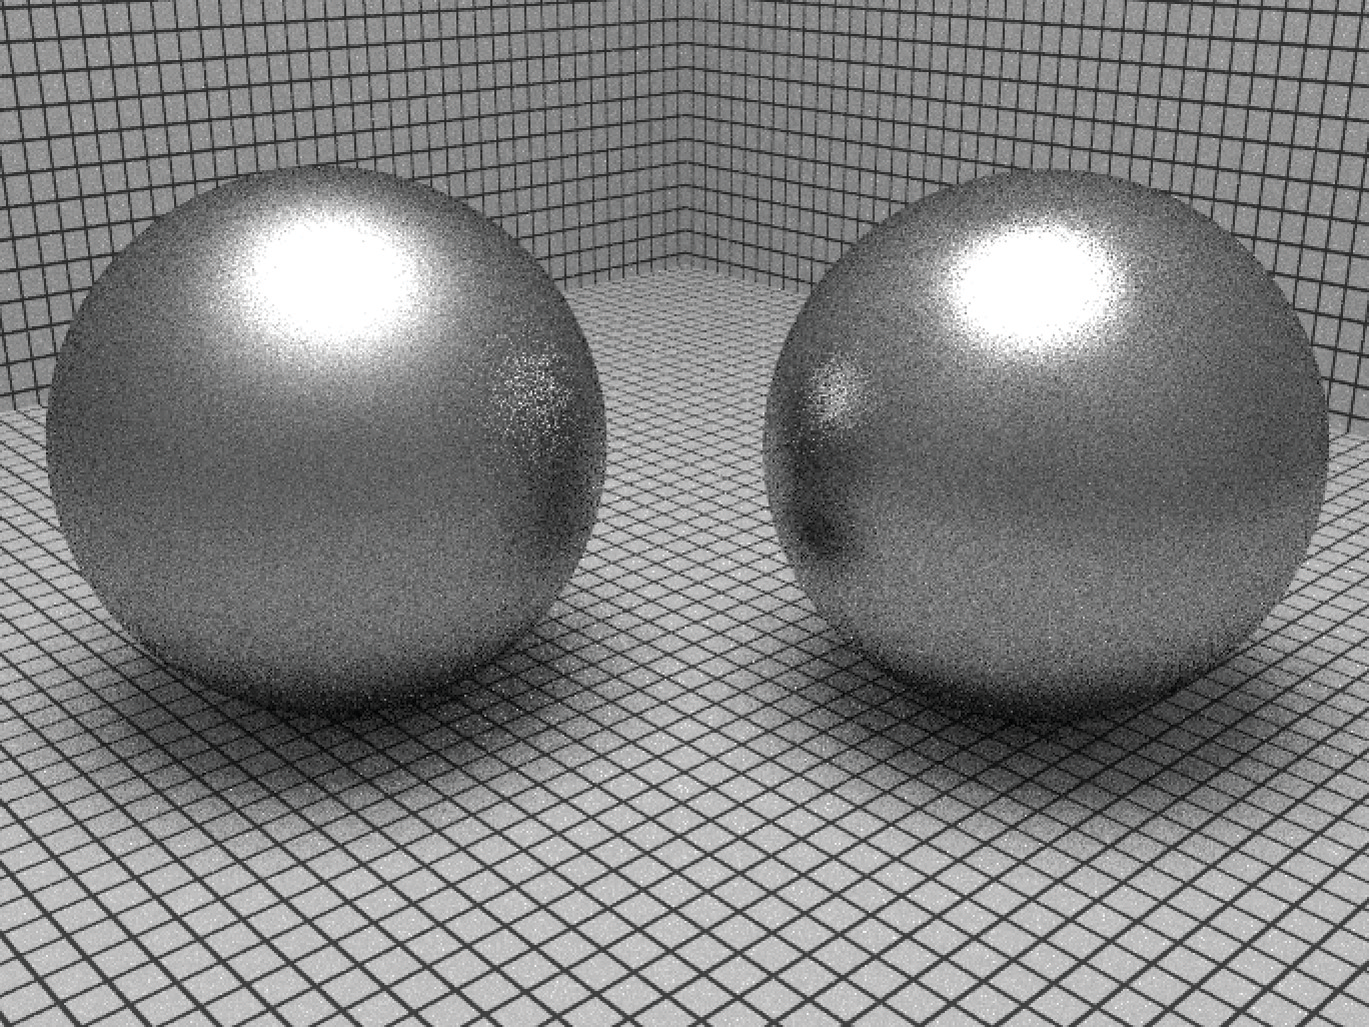
\includegraphics[width=\linewidth]{chap07/spheres-bad-sampler.png}\label{fig:7.14.1}}\\
    \subfloat[更好的采样]{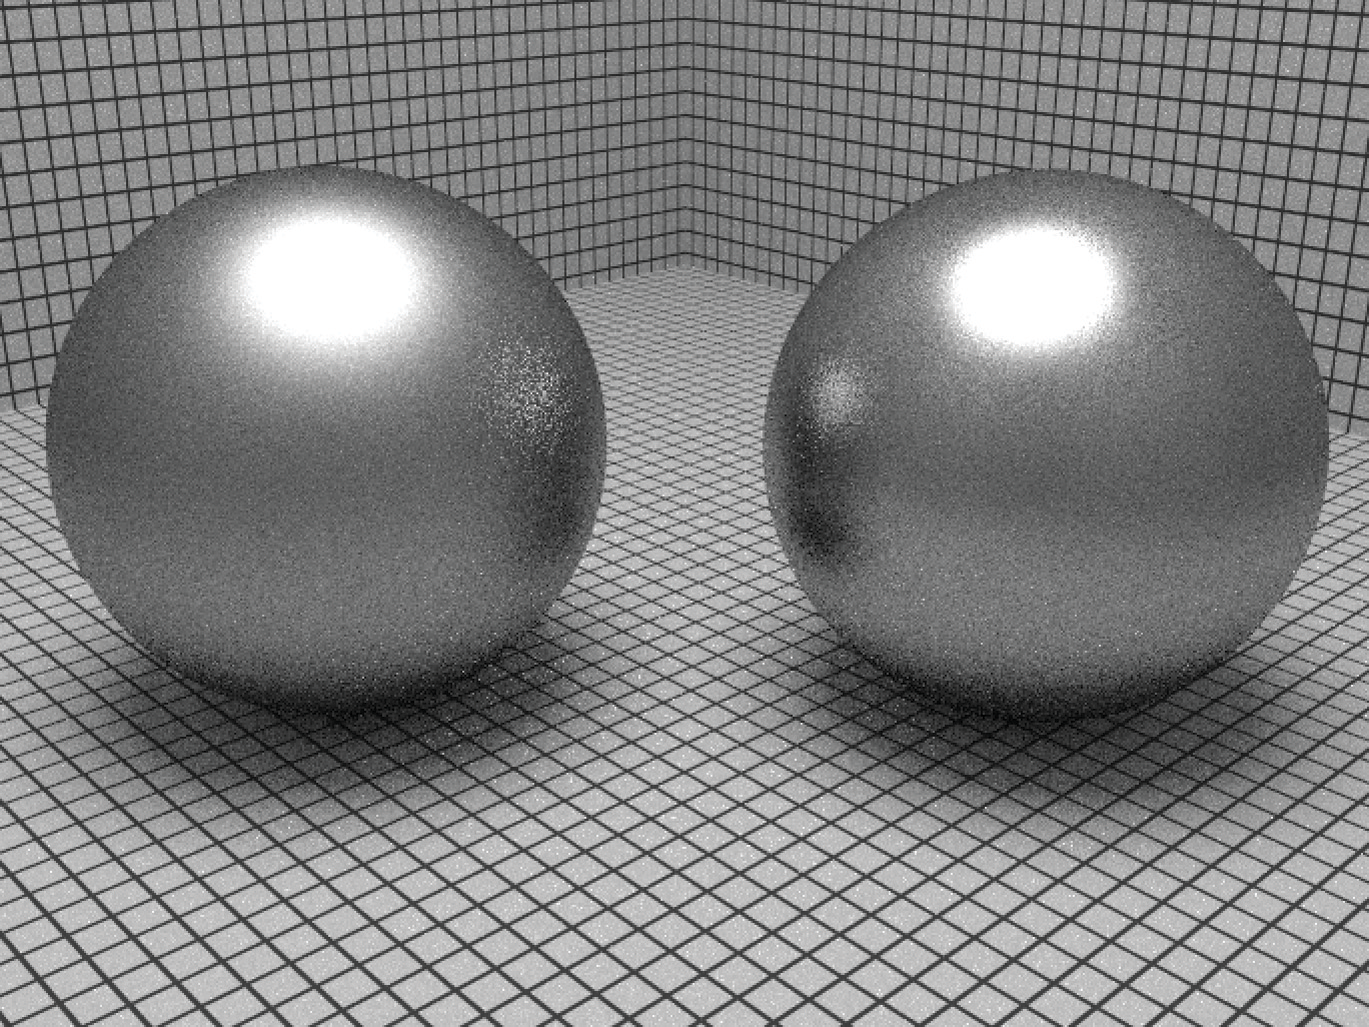
\includegraphics[width=\linewidth]{chap07/spheres-better-sampler.png}\label{fig:7.14.2}}
    \caption{用(a)相对低效的采样器和(b)精心设计的采样器渲染的场景,
        它们用了同样多的样本。从高光边缘到光泽反射,图像质量的提升是明显的。}
    \label{fig:7.14}
\end{figure}

下面假设这些样本向量的一些特性:
\begin{itemize}
    \item \refvar{Sampler}{}生成的前五维通常由\refvar{Camera}{}使用。
          这种情况下,前两个专门用于选择图像上当前像素区域内的点;
          第三个用于计算应该取用该样本的时间;第四和五维为景深给出透镜位置$(u,v)$。
    \item 一些采样算法在样本向量的某些维度中生成的样本比其他维度更好。
          在系统其他地方,我们假设一般前面的维度具有放置得最好的样本值。
\end{itemize}

还要注意\refvar{Sampler}{}生成的$n$维样本通常不会整个显式表示或存储,
而是常常按照光传输算法的需要逐步生成。(然而,存储整个样本向量并对其分量逐渐作出调整
是\refsub{基本样本空间采样器}中\refvar{MLTSampler}{}的基础,
它用于\refsub{MLT积分器}的\refvar{MLTIntegrator}{}。)

\subsection{评估样本模式:偏差}\label{sub:评价样本模式:偏差}
\begin{remark}
    本节含有高级内容,第一次阅读时可以跳过。
\end{remark}

傅里叶分析给了我们一种方法来评估2D采样模式的质量,
但它只是让我们能够在可表示的带限频率方面量化增加更均匀间隔的样本所带来的提升。
考虑到图像中出现了来自边缘的无穷频率成分以及蒙特卡罗光传输算法对$(n>2)$维样本向量的需求,
傅里叶分析对于我们的需求而言是不够的。

给定一个渲染器和放置样本的候选算法,一种评估该算法效果的方法是用其
采样模式来渲染图像并计算它和用大量样本渲染的参考图像相比的误差。
本章后面我们将用该方法比较采样算法,不过它只告诉了我们该算法对于特定场景的表现如何,
且若没有经过渲染过程它将不能让我们感觉出样本点的质量。

除了傅里叶分析,数学家还发明了一个称作\keyindex{偏差}{discrepancy}{}的概念
用于评估$n$维样本位置模式的质量。分布良好(稍后形式化说明)的模式有低的偏差值,
且因此该样本模式生成问题可以考虑成寻找点的合适的\emph{低偏差}模式
\footnote{当然,这样使用偏差隐含假设了用于计算偏差的度量
    对于图像采样而言是与模式的质量有良好关联性的,这可能会有所区别,
    尤其是当人类视觉系统参与该过程时。}。
大量确定性技术已经被开发出来,甚至能在高维空间中生成低偏差点集
(本章后面所用的大多数采样算法都使用这些技术)。

偏差的基本思想是$n$维空间$[0,1)^n$中点集的质量可通过查看域$[0,1)^n$中的各区域、
数出每个区域内的点数并拿每个区域的体积和其内的样本点数作比较来评估。
通常,给定的某一占比体积内应该大致含有样本点总数的相同比例。
尽管不可能总是这种情况,但我们仍可尽量使用让实际体积与点估计的体积间的最大差异(即偏差)最小化的模式。
\reffig{7.15}展示了该思想在二维下的例子。
\begin{figure}[htbp]
    \centering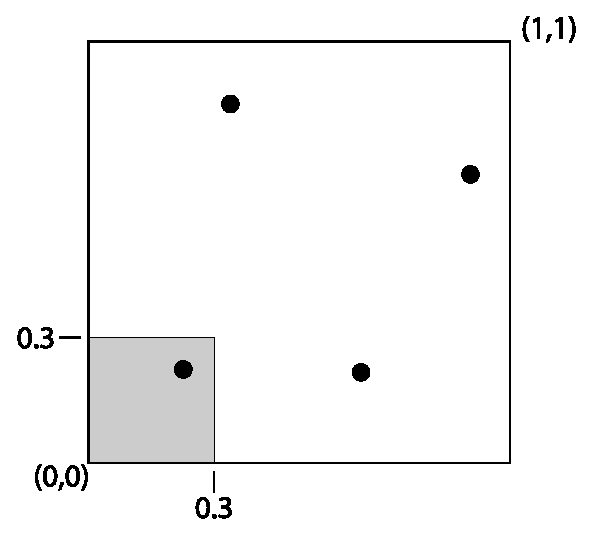
\includegraphics[width=0.5\linewidth]{chap07/Boxdiscrepancy.eps}
    \caption{给定$[0,1)^2$中2D样本点集后矩形(阴影)的偏差。
    四个样本点中的一个在矩形内,所以该点集将把矩形的面积估为$\frac{1}{4}$。
    该矩形是真实面积是$0.3\times0.3=0.09$,所以该特定矩形的偏差
    为$0.25-0.09=0.16$。通常,我们关心的是找出所有可能的矩形(或某些其他形状)中的最大偏差。}
    \label{fig:7.15}
\end{figure}

为了计算点集的偏差,我们首先取作为$[0,1)^n$子集的一簇形状$B$。
例如常用一个角位于原点的方盒。其对应于
\begin{align*}
    B=\{[0,v_1]\times[0,v_2]\times\cdots\times[0,v_n]\}\, ,
\end{align*}
其中$0\le v_i<1$。给定样本点序列$P=x_1,\ldots,x_N$,
$P$关于$B$的偏差为\footnote{算符$\sup$,也称作\emph{上确界},给出了定义域内函数值的最紧上界。}
\begin{align}\label{eq:7.4}
    D_N(B,P)=\sup\limits_{b\in B}\left|\frac{\#\{x_i\in b\}}{N}-V(b)\right|\, ,
\end{align}
其中$\#\{x_i\in b\}$是$b$中的点数,$V(b)$是$b$的体积。

对于为什么\refeq{7.4}是合理的质量度量的直观解释是,
值$\displaystyle\frac{\#\{x_i\in b\}}{N}$是
由特定点集$P$给出的方盒$b$体积的近似。
因此,偏差是所有可能的方盒用这种办法逼近其体积时的最差误差。
当形状集$B$是一个角在原点的方盒集时,
该值称为\keyindex{星偏差}{star discrepancy}{discrepancy偏差}
\sidenote{译者注:也称“均匀性偏差”。},$D^*_N(P)$。
对于$B$的另一个流行选择是全体轴对齐框的集合,即去掉了一个角在原点的限制。

对于一些特定点集,可以解析计算偏差。例如考虑一维中的点集
\begin{align*}
    x_i=\frac{i}{N}\, .
\end{align*}
我们可以看到$x_i$的星偏差为\sidenote{译者注:原文将$x_N$误写为$x_n$,已修正。}
\begin{align*}
    D^*_N(x_1,\ldots,x_N)=\frac{1}{N}\, .
\end{align*}
例如,取区间$b=\displaystyle\left[0,\frac{1}{N}\right)$。则$V(b)=\displaystyle\frac{1}{N}$,
但$\#\{x_i\in b\}=0$。该区间(以及区间$\displaystyle\left[0,\frac{2}{N}\right)$等)
的体积与体积内所见点的比例有最大的差异。

该序列的星偏差可通过稍微对其改动来改进:
\begin{align}\label{eq:7.5}
    x_i=\frac{i-\frac{1}{2}}{N}\, .
\end{align}
则
\begin{align*}
    D^*_N(x_i)=\frac{1}{2N}\, .
\end{align*}
说明一维点序列的星偏差边界为
\sidenote{译者注:这里我简单推导了该式:假设$P=\{x_i\}_{i=1}^{N}$已经按照
升序排列。构造一个新序列$Q=\left\{\frac{j}{N}\right\}_{j=0}^{N}$,然后让$P$和$Q$的元素交错排列构造
新序列$U=\{u_k\}_{k=1}^{2N+1}=\left\{0,x_1,\frac{1}{N},\ldots,x_i,\frac{i}{N},\ldots,x_N,1\right\}$。
则依据偏差的定义可以证明,$D^*_N(x_i)=\max\limits_{1\le k\le 2N}{|u_{k+1}-u_k|}=\max\limits_{1\le i\le N}{d_i}$,
其中$d_i=\max{\left\{\left|x_i-\frac{i-1}{N}\right|,\left|x_i-\frac{i}{N}\right|\right\}}$。
又注意到$d_i=\frac{1}{2N}+\left|x_i-\frac{2i-1}{2N}\right|$,于是得到文中该式。}
\begin{align*}
    D^*_N(x_i)=\frac{1}{2N}+\max\limits_{1\le i\le N}\left|x_i-\frac{2i-1}{2N}\right|\, .
\end{align*}
因此,之前\refeq{7.5}中的序列具有1D序列中所能取到的最低偏差。
通常,分析和计算1D序列的偏差边界比高维简单得多。
对于构造更复杂的点序列、高维序列以及比方盒更不规则的形状,
通常必须通过构造大量形状$b$、计算其偏差并报告找到的最大值来数值地估计偏差。

聪明的读者会注意到根据低偏差度量,1D中该均匀序列是最优的,
但本章前面我们说过,对于2D中的图像采样,不规则的抖动模式优于均匀模式,
因为它们将混叠替换为噪声。在这一框架下,均匀样本显然不是最好的。
幸运的是,更高维的低偏差模式比在一维中更不均匀得多,
因此实际中通常能作为样本模式工作得很好。
然而,其根本的均匀性意味着低偏差模式比伪随机变化的模式更可能倾向于视觉上令人讨厌的混叠。

只靠偏差并不一定是好的度量:一些低偏差点集表现出样本的聚集性,
其中两个或以上样本可能靠得很近。\refsec{Sobol采样器}的Sobol采样器
尤其困扰于该问题——见\reffig{7.36},它展示了其前两维的图示。
直觉上,靠得太近的样本不能很好地利用采样资源:
一个样本离另一个越近,它就越不可能给出关于被采样函数的新信息。
因此,计算点集中任意两个样本间的最小距离也已被证明是一种有用的样本模式质量度量;最小距离越大越好。

有各种算法用来生成在该度量下得分不错的\keyindex{泊松圆盘}{Poisson disk}{}采样模式。
通过构造,泊松圆盘模式内没有两个点比某一距离$d$更近。
研究已表明眼睛的视杆细胞和视锥细胞也按该方式分布,
这进一步验证了该分布适合用来成像的观点。
实际中,我们发现泊松圆盘模式对于采样2D图像工作得很好,
但对于更复杂的渲染情形中的更高维采样会比更好的低偏差模式更低效;
见“扩展阅读”一节了解更多信息。

\subsection{基本采样器接口}\label{sub:基本采样器接口}
基类\refvar{Sampler}{}不仅定义了采样器的接口,
还提供了一些通用功能供\refvar{Sampler}{}
的实现使用。
\begin{lstlisting}
`\initcode{Sampler Declarations}{=}\initnext{SamplerDeclarations}`
class `\initvar{Sampler}{}` {
public:
    `\refcode{Sampler Interface}{}`
    `\refcode{Sampler Public Data}{}`
protected:
    `\refcode{Sampler Protected Data}{}`
private:
    `\refcode{Sampler Private Data}{}`
};
\end{lstlisting}

所有\refvar{Sampler}{}实现必须提供指定了要为最终图像中每个像素生成的样本数量的构造函数。
在罕见情况下,将胶片建模为只有单个覆盖整个可视区域的“像素”可能对系统有用
(这种过载的像素定义有点夸张,但我们允许它简化某些实现方面)。
既然该“像素”可能有数十亿个样本,我们就用64位精度的变量来存储样本数量。
\begin{lstlisting}
`\initcode{Sampler Method Definitions}{=}\initnext{SamplerMethodDefinitions}`
`\refvar{Sampler}{}`::`\refvar{Sampler}{}`(int64_t samplesPerPixel)
: `\refvar{samplesPerPixel}{}`(samplesPerPixel) { }
\end{lstlisting}
\begin{lstlisting}
`\initcode{Sampler Public Data}{=}`
const int64_t `\initvar{samplesPerPixel}{}`;
\end{lstlisting}

当渲染算法准备好在给定像素上工作时,它通过提供
该像素在图像中的坐标并调用\refvar{StartPixel}{()}来开始。
一些\refvar{Sampler}{}实现利用哪个像素正被采样的知识来提升
其为该像素生成的样本整体分布,而其他的则忽略该信息。
\begin{lstlisting}
`\initcode{Sampler Interface}{=}\initnext{SamplerInterface}`
virtual void `\initvar{StartPixel}{}`(const `\refvar{Point2i}{}` &p);
\end{lstlisting}

方法\refvar{Get1D}{()}为当前样本向量的下一维返回样本值,
\refvar{Get2D}{()}则为下两维返回样本值。
尽管能通过使用调取一对\refvar{Get1D}{()}返回的值来构造2D样本值,
但一些采样器如果知道两维会一起用时能够生成更好的点分布。
\begin{lstlisting}
`\refcode{Sampler Interface}{+=}\lastnext{SamplerInterface}`
virtual `\refvar{Float}{}` `\initvar{Get1D}{}`() = 0;
virtual `\refvar{Point2f}{}` `\initvar{Get2D}{}`() = 0;
\end{lstlisting}

在pbrt中,我们不支持从采样器中获取3D或更高维度的样本值,
因为它们一般对于这里实现的渲染算法类型而言是非必需的。
如果需要,可用来自低维分量的多个值来构造高维样本点。

这些接口的一个显著特点是必须仔细编写使用样本值的代码使其
总是以同样的顺序获取样本维度。考虑下列代码:\\
{\ttfamily
sampler->StartPixel(p);\\
do \{\\
        \indent Float v = a(sampler->Get1D());\\
        \indent if (v > 0)\\
        \indent \indent v += b(sampler->Get1D());\\
        \indent v += c(sampler->Get1D());\\
\} while (sampler->StartNextSample());
}

情况下,样本向量的第一维总会传给函数{\ttfamily a()};
当执行调用{\ttfamily b()}的代码路径时,{\ttfamily b()}会收到第二维。
然而,若{\ttfamily if}测试并不总是为真或假,则{\ttfamily c()}有时
会从样本向量的第二维收到样本,否则从第三维收到样本。
因此,采样器为了提供在每个维度评估都分布良好的样本点所作的努力就白费了。
故需要仔细编写使用\refvar{Sampler}{}的代码使得它始终如一地用掉样本向量维度以避免该问题。

为了方便,基类\refvar{Sampler}{}提供了为给定像素初始化\refvar{CameraSample}{}的方法。
\begin{lstlisting}
`\refcode{Sampler Method Definitions}{+=}\lastnext{SamplerMethodDefinitions}`
`\refvar{CameraSample}{}` `\refvar{Sampler}{}`::`\initvar{GetCameraSample}{}`(const `\refvar{Point2i}{}` &pRaster) {
    `\refvar{CameraSample}{}` cs;
    cs.`\refvar{pFilm}{}` = (`\refvar{Point2f}{}`)pRaster + `\refvar{Get2D}{}`();
    cs.`\refvar[CameraSample::time]{time}{}` = `\refvar{Get1D}{}`();
    cs.`\refvar{pLens}{}` = `\refvar{Get2D}{}`();
    return cs;
}
\end{lstlisting}

一些渲染算法为其采样的某些维度利用了样本值数组;
比起生成一系列单独的样本,大多数样本生成算法通过考虑
数组所有元素上以及一个像素内所有样本上的样本值分布可生成更高质量的样本数组。

如果需要样本数组,则必须在渲染开始前请求之。
在渲染开始前——例如在重写了方法\refvar{SamplerIntegrator::Preprocess}{()}的方法中,
应该为每个这样维度的数组调用方法\refvar[Request1DArray]{Request[12]DArray}{()}。
例如,在具有两个面光源的场景中,当积分器追踪了四条阴影射线到第一个光源,
八条到第二个光源时,积分器会为每个图像样本请求两个2D样本数组,
每个分别有四个和八个样本(需要2D数组是因为需要两个维度来参数化光源表面)。
在\refsec{俄罗斯轮盘赌与划分}中,我们将看到使用样本数组会怎样对应于
用“划分”\sidenote{译者注:原文splitting。}的蒙特卡罗技术更密集地采样光传输积分的某些维度。
\begin{lstlisting}
`\refcode{Sampler Interface}{+=}\lastnext{SamplerInterface}`
void `\initvar{Request1DArray}{}`(int n);
void `\initvar{Request2DArray}{}`(int n);
\end{lstlisting}

大多数\refvar{Sampler}{}能更好地生成某些特定大小的数组。
例如,在数量为2的幂时,来自\refvar{ZeroTwoSequenceSampler}{}的样本则分布得好得多。
方法\refvar[RoundCount]{Sampler::RoundCount}{()}
帮助传达该信息。需要样本数组的代码应该用想要取用的样本数目调用该方法,
以给\refvar{Sampler}{}机会把样本数目调整到更好的值。
然后应该用返回的值作为从\refvar{Sampler}{}实际请求样本的数目。
默认实现返回不变的给定数目。
\begin{lstlisting}
`\refcode{Sampler Interface}{+=}\lastnext{SamplerInterface}`
virtual int `\initvar{RoundCount}{}`(int n) const {
    return n;
}
\end{lstlisting}

在渲染时,可调用方法\refvar[Get1DArray]{Get[12]DArray}{()}获取
指向之前请求的当前维度下样本数组起点的指针。
在\refvar{Get1D}{()}和\refvar{Get2D}{()}的代码行中,
它们返回指向样本数组的指针,数组大小由参数{\ttfamily n}传给
初始化时对\refvar[Request1DArray]{Request[12]DArray}{()}的相应调用。
调用者还必须提供数组大小以“获取”方法用于验证返回的缓冲区具有期望大小。
\begin{lstlisting}
`\refcode{Sampler Interface}{+=}\lastnext{SamplerInterface}`  
const `\refvar{Float}{}` *`\initvar{Get1DArray}{}`(int n);
const `\refvar{Point2f}{}` *`\initvar{Get2DArray}{}`(int n);
\end{lstlisting}

为一个样本完成这些工作后,积分器调用\refvar{StartNextSample}{()}。
该调用为当前像素通知\refvar{Sampler}{}针对
样本分量的后续请求应该返回下一个样本从第一维起的值。
该方法返回{\ttfamily true},直到已经为每个像素生成了请求的原始数目样本
(此时调用者应该要么在另一个像素上开始工作要么停止试图使用更多样本)。
\begin{lstlisting}
`\refcode{Sampler Interface}{+=}\lastnext{SamplerInterface}`
virtual bool `\initvar{StartNextSample}{}`();
\end{lstlisting}

\refvar{Sampler}{}的实现存储了关于当前样本的各种状态:
正在采样哪个像素,用了该样本的多少维度等等。
因此对于多个线程同时使用的单个\refvar{Sampler}{}而言自然是不安全的。
方法\refvar{Clone}{()}生成一个初始\refvar{Sampler}{}的新实例给渲染线程使用;
它为采样器的随机数生成器(如果有)接收一个种子值,这样不同线程会有不同的随机数序列。
在多个图块间复用相同伪随机数序列可能导致微妙的图像伪影,例如重复的噪声模式。

方法\refvar{Clone}{()}的各种实现一般并不有趣,所以这里文中没有包含它们。
\begin{lstlisting}
`\refcode{Sampler Interface}{+=}\lastnext{SamplerInterface}`
virtual std::unique_ptr<`\refvar{Sampler}{}`> `\initvar{Clone}{}`(int seed) = 0;
\end{lstlisting}

一些光传输算法(特别是\refsec{随机渐进光子映射}的随机渐进光子映射)
在进行到下一像素前并不使用当前像素内的所有样本,
而是跳跃到周围的像素,每个里面每次取一个样本。
方法\refvar{SetSampleNumber}{()}允许积分器在当前像素内设置样本的索引以生成下一个。
一旦{\ttfamily sampleNum}大于或等于每个像素请求的原始样本数目该方法就返回{\ttfamily false}。
\begin{lstlisting}
`\refcode{Sampler Interface}{+=}\lastcode{SamplerInterface}`
virtual bool `\initvar{SetSampleNumber}{}`(int64_t sampleNum);
\end{lstlisting}

\subsection{采样器实现}\label{sub:采样器实现}
基类\refvar{Sampler}{}在其接口内提供了一些方法的实现。